\documentclass[a5paper, 10pt, twoside, onecolumn, openany]{memoir}
\usepackage{hegel}
\usepackage{multicol}

\hypersetup{
  pdfborder={0 0 0},    % No borders around internal hyperlinks
  pdfauthor={ФРА}       % author
}

\author{Г.~В.~Ф. Гегель}
\title{Наука логики}
\date{}

\begin{document}

\frontmatter
\thispagestyle{plainfullpagecover}

{\centering\color{white}
  {\Large Г.~В.~Ф.~ГЕГЕЛЬ} \\
  \vspace{45mm+29mm}
  \textbf{\Huge НАУКА ЛОГИКИ} \\
  \vspace{6mm}
  {\Large Том~I. Объективная логика} \\
  \vspace{2mm}
  {\large Книга~I. Учение о~бытии} \\
  \vspace{25mm+16mm}
  \textit{перевод} \\
  \textit{Б.~Г.~СТОЛПНЕРА} \\
  \vspace{2mm}
  \textit{под редакцией} \\
  \textit{М.~Б.~МИТИНА}
\par}

\let\leftmarkold\leftmark
\renewcommand\leftmark{\memUChead{Г.В.Ф. Гегель. Наука логики. Том I. Книга 1}}


%\cleardoublepage
\clearpage
\thispagestyle{bookoutput}
{\small
\noindent\textbf{Гегель, Г.~В.~Ф.}\newline
\textbf{Наука логики. Том~I. Объективная логика, Книга~1. Учение о~бытии.}
[пер. с~нем. Б.~Г.~Столпнера. Сверено с~изданиями 1970 и~2005~годов, а~также
с~немецким оригиналом]. "--- ПК~«Советская типография», Международное
сообщество Текнокомо, 2025 "--- 504~с.\vspace{2ex}

{\setlength\parskip{0mm}
<<Наука логики>> "--- важнейшее сочинение Гегеля, где рельефно выступает его
диалектический метод. Классики марксизма"=ленинизма высоко ценят этот труд
Гегеля.

Ленин писал, что <<нельзя вполне понять <<Капитала>> Маркса и~особенно его
I~главы, не~проштудировав и~не~поняв всей Логики Гегеля>>. Гегель угадал
диалектику вещей в~диалектике понятий. Диалектика Гегеля идеалистична, поэтому
Ленин писал:<<Логику Гегеля нельзя применять в~данном её~виде; нельзя брать как
данное. Из~неё надо выбрать логические (гносеологические) оттенки, очистив
от~мистики идей: это ещё большая работа».

<<Наука логики>> Гегеля даётся в новом переводе.}}

\vspace{1ex}
{\footnotesize\noindent
Главный редактор: \textit{М.~В.~Попов}\newline
Координатор сверки: \textit{Артур Ефимов}\newline
Механизация: \textit{Артур Ефимов, Даниэль Высоцкий}\newline
Вёрстка: \textit{Артур Ефимов, Даниэль Высоцкий, Сергей Пеганов}\newline
Художественное оформление: \textit{Патрик Александрян, Сергей Лавренюк}\newline
Производство: \textit{Юлия Редина, Михаил Сергеев}

\vspace{-0.5ex}
\begin{multicols}{3}[\noindent Вычитка:\vspace{-3.25ex}]
  \noindent\emАлександр Алексеев\newline
  Алексей Брызгалов\newline
  Александр Букин\newline
  Андрей Кулаго\newline
  Андрей Марсов\newline
  Артур Ефимов\newline
  Даниэль Высоцкий\newline
  Дмитрий Воронович\newline
  Евгений Зеленков\newline
  Елена Корнетова\newline
  Иван Бабак\newline
  Михаил Медвецкий\newline
  Михаил Сергеев\newline
  Никита Зырянов\newline
  Никита Прокопенко\newline
  Олег Биркис\newline
  Патрик Александрян\newline
  Сергей Пеганов\newline
  Сергей Пушкарев\newline
  Сергей Яранов\newline
  Сергей Шукшин\newline
  София Воронка\newline
  Эдуард Мукан\newline
  Юлия Редина
\end{multicols}
\vspace{-4ex}
\begin{multicols}{3}[\noindent Особые благодарности:\vspace{-3.25ex}]
  \noindent\em
  Александр Савин\newline
  Александр Миненков\newline
  Андрей Вржещ\newline
  Андрей Патин\newline
  Артём Прокопович\newline
  Василий Манжула\newline
  Ивайло Иванов\newline
  Павел Перов\newline
  Роман Пузанков\newline
  Руслан Богатырев\newline
  \textls[-50]{Фонд Рабочей Академии}\newline
  \textls[-50]{Рабочий фронт Латвии}\newline
  \textls[-50]{Красный Университет}\newline
  \textls[-80]{ПК <<Советские роботы>>}
\end{multicols}
\vspace{-4.0ex}
\noindentГенеральный разнорабочий: \textit{Владимир Левадный}

\vfil
\noindent\textbf{Пилотный экземпляр}\vspace{-2.5ex}
}
\clearpage

\pagestyle{simple}
\pagenumbering{Roman}
\setcounter{page}{1}
\renewcommand{\parttitlefont}{\Huge\color{white}}
\input{001_o_znachenii.tex}

\cleardoublepage

\mainmatter
\thispagestyle{plainfullpagecover}
{\centering\color{white}
  \ \\
  \vspace{50mm}
  {\huge\bfseries ГЕГЕЛЬ} \\
  \vspace{50mm}
  {\Huge\bfseries НАУКА ЛОГИКИ}
\par}

\addtocontents{toc}{\vspace{3mm}%
  {\centering%
    \normalsize\bfseries\em Гегель <<НАУКА ЛОГИКИ>>\\%
  }%
  \vspace{1mm}}

\newgeometry{left=15mm,right=15mm,top=25mm,bottom=5mm}
\thispagestyle{plainfullpagecover}
\begin{center}
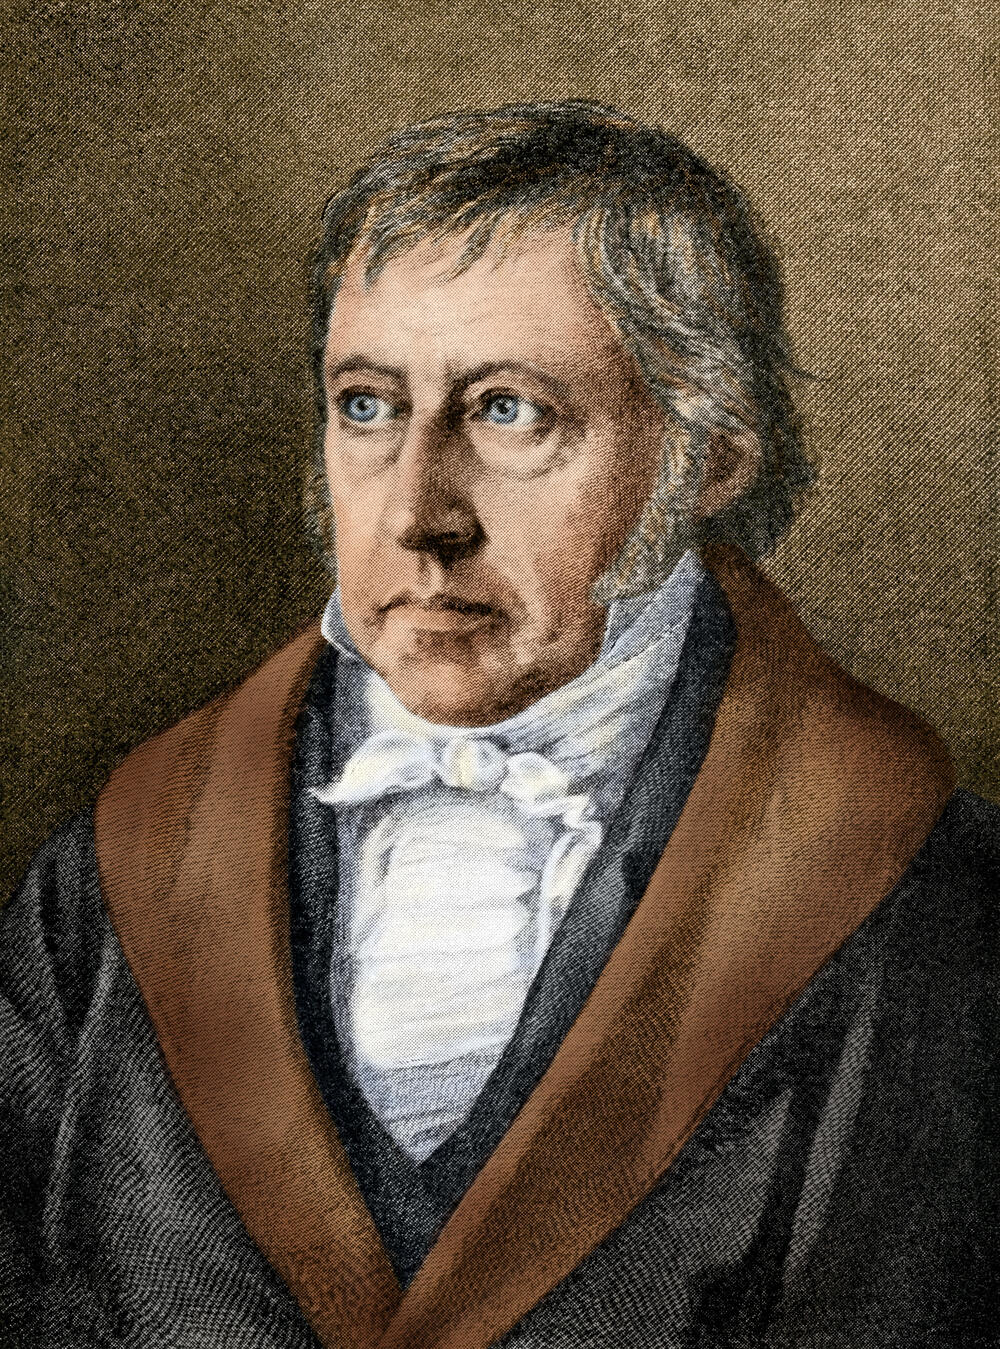
\includegraphics[width=11.4cm]{hegel-img001.png}
\end{center}

\restoregeometry

\setsecnumdepth{none}
\chapter[Предисловие к~первому изданию]{\large ПРЕДИСЛОВИЕ К~ПЕРВОМУ ИЗДАНИЮ}
\input{002_predislovie.tex}

\clearpage

\chapter[Предисловие ко второму изданию]{\large ПРЕДИСЛОВИЕ КО ВТОРОМУ ИЗДАНИЮ}
\input{003_predislovie.tex}

\clearpage

\chapter[Введение]{ВВЕДЕНИЕ}
\input{004_vvedenie.tex}

\addtocontents{toc}{\vspace{7mm}%
  {\centering\lsstyle\normalsize\bfseries Первая книга\\}%
   \vspace{2mm}}

\part[УЧЕНИЕ О~БЫТИИ]%
     {\ \\\vspace{10mm}\Large\mdseries ПЕРВАЯ КНИГА\\\ \\
     \Huge\bfseries УЧЕНИЕ О~БЫТИИ}
\addtocspace{2mm}

\setsecnumdepth{subsection}
\subsubsection{С~чего следует начинать науку}
\let\rightmarkold\rightmark
\renewcommand\rightmark{\memUChead{С~чего следует начинать науку}}
\input{101_s_chego.tex}

\setsecnumdepth{subsubsection}
\chapter[Определённость (качество)]{Определённость\\(качество)}
\renewcommand\rightmark\rightmarkold

% Первая глава. Бытие.
\input{111_bytie.tex}

\section{Наличное бытие}
\input{112_nalichnoe_bytie.tex}

\section{Для-себя-бытие}
\input{113_dlya_sebya_bytie.tex}

\chapter[Величина (количество)]{Величина\\(количество)}

% Первая глава. Количество.
\input{121_kolichestvo.tex}

\section{Определённое количество}
\input{122_opredelyonnoe_kolichestvo.tex}

\section{Количественное отношение}
\input{123_kolichestvennoe_otnoshenie.tex}

\chapter{Мера}

% Первая глава. Специфическое количество.
\input{131_specificheskoe_kolichestvo.tex}

\section{Реальная мера}
\input{132_realnaya_mera.tex}

\section{Становление сущности}
\input{133_stanovlenie_suschnosti.tex}

\backmatter

\addtocontents{toc}{\vspace{6mm}%
  {\centering\normalsize\bfseries ПРИЛОЖЕНИЯ\\}}

\renewcommand\appendixpagename{\ \vspace{16mm}\par\HUGE\bfseriesПРИЛОЖЕНИЯ}
\appendixpage*

% Предисловие издателя (Леопольда фон Геннинга)
\input{141_prilozhenija.tex}

\chapter[\mdseries Примечания]{ПРИМЕЧАНИЯ}
\input{142_primechanija.tex}

\clearpage
\tableofcontents*
\clearpage

\end{document}
